\documentclass[a4paper, 12pt, final, garamond]{book}
\usepackage{cours-preambule}

\raggedbottom

\makeatletter
\renewcommand{\@chapapp}{M\'ecanique -- chapitre}
\makeatother

\begin{document}
\setcounter{chapter}{2}

\chapter{Correction TD application}
\section{Projection de vecteurs}
\begin{enumerate}
    \item Si $\a$ vaut 0, $\vfo$ est selon $\ux$. On sait donc que la
        projection de $\vfo$ sur $\ux$ donne $v_0\cos\a\ux$. On le remarque
        également avec le triangle rectangle OMH, avec M le bout de $\vfo$ et H
        son projeté orthogonal sur $\ux$~: la longueur OH est en effet
        $v_0\cos\a$. \bigbreak
        Si $\a$ vaut $\pi/2$, $\vfo$ est selon $\uz$. On sait donc que la
        projection de $\vfo$ sur $\uz$ donne $v_0\sin\a\uz$. On le remarque
        également en prenant le triangle rectangle OMJ, avec cette fois J le
        projeté orthogonal de M sur $\uz$~: la longueur OJ est en effet
        $v_0\sin\a$. Finalement,
        \[\boxed{\vfo = v_0\cos\a\ux + v_0\sin\a\uz}\]
    \item Avec la même réflexion, on trouve
        \[\boxed{\Tf = T\cos\a\ux + T\sin\a\uz}\]
        La méthode est la même pour $\Nf$, mais le résultat est différent. En
        effet, si $\a = 0$, $\Nf$ est selon $\uz$~: la projection de $\Nf$ sur
        $\uz$ donne $N\cos\a\uz$. Si $\a = \pi/2$, $\Nf$ est selon $-\ux$~: la
        projection de $\Nf$ sur $\ux$ donne $-N\sin\a\ux$. Ainsi,
        \[\boxed{\Nf = -N\sin\a\ux + N\cos\a\uz}\]

    \item Toujours même réflexion~: si $\tt = 0$, $\Pf$ est selon $\er$, et si
        $\tt = \pi/2$, $\Pf$ est selon $-\et$. $\Tf$ est, par définition, selon
        $-\er$. Ainsi,

        \[
            \boxed{\Pf = mg\cos\tt\er -mg\sin\tt\et}
            \qet
            \boxed{\Tf = -T\er}
        \]
    \item Ici aussi~:
        \begin{itemize}
            \item $\a = 0 \Ra \Pf\cdot\vv{e_Y} = -1
                        \quad
                        \text{($\Pf$ selon $-\vv{e_Y}$)}$
            \item $\a = \pi/2 \Ra
                        \Pf\cdot\vv{e_X} = 1
                        \quad
                        \text{($\Pf$ selon $\vv{e_X}$)}$
        \end{itemize}
        Ainsi
        \[
            \boxed{\Pf = mg(\sin\a\vv{e_X} -\cos\a\vv{e_Y})}
            \qet
            \boxed{\Nf = N\vv{e_Y}}
            \qet
            \boxed{\Tf = -T\vv{e_X}}
        \]
        D'où
        \[
            \Nf + \Tf + \Pf = \of
            \Lra
            \mqty(mg\sin\a -T\\-mg\cos\a + N) = \mqty(0\\0)
            \Lra
            \boxed{
            \left\{
                \begin{aligned}
                    T &= mg\sin\a\\
                    N &= mg\cos\a
                \end{aligned}
            \right.}
        \]
    \item On projette~:
        \[
            \Ff_g = F_g(\cos\a\uy -\sin\a\ux)
            \qet
            \Ff_d = F_d(\cos\bb\uy+\sin\bb\ux)
        \]
        et avec l'égalité de vecteurs on obtient
        \begin{align*}
            \left\{
                \begin{aligned}
                    0 & = F_d\sin\bb -F_g\sin\a\\
                    0 & = -mg+F_g\cos\a + F_d\cos\bb
                \end{aligned}
            \right.
            &\Lra
            \left\{
                \begin{aligned}
                    F_d & = F_g\frac{\sin\a}{\sin\bb}\\
                    mg  & = F_g\cos\a + F_g\frac{\sin\a}{\sin\bb}\cos\bb
                \end{aligned}
            \right.
            \\\Lra
            \left\{
                \begin{aligned}
                    F_d       & = F_g\frac{\sin\a}{\sin\bb}\\
                    mg\sin\bb & = F_g(\cos\a\sin\bb + \sin\a\cos\bb)
                \end{aligned}
            \right.
            &\Lra
            \boxed{
            \left\{
                \begin{aligned}
                    F_d & = \frac{mg\sin\a}{\cos\a\sin\bb + \sin\a\cos\bb}\\
                    F_g & = \frac{mg\sin\bb}{\cos\a\sin\bb + \sin\a\cos\bb}
                \end{aligned}
            \right.
            }
        \end{align*}
        Les applications numériques, \textbf{non demandées}, donnent
        \[
            \boxed{
            \left\{
                \begin{array}{rcl}
                    F_d & = & \SI{4.4e2}{N}\\
                    F_g & = & \SI{5.4e2}{N}
                \end{array}
            \right.
            }
        \]
\end{enumerate}

\section{Masse du Soleil}
On étudie le système \{Terre\} dans le référentiel héliocentrique. La Terre
étant sur une orbite circulaire, on utilise un repère polaire $({\rm
S},\ur,\ut)$ en appelant S le centre de gravité du
Soleil et T le centre de gravité de la Terre. On a~:
\begin{gather*}
    \vv{\rm ST} = R\ur\\
    \vf = R\tp\ut\\
    \af = \underbrace{\cancel{R\tpp\ut}}_{\tpp=0} -R\tp^2\ur
\end{gather*}
étant donné que la distance Terre-Soleil est fixe, et que la vitesse angulaire
de la Terre autour du Soleil est constante. On a d'ailleurs, en appelant $\w =
\tp$ cette vitesse angulaire,
\[\w = \frac{2\pi}{T_0}\]
avec $T_0$ la période de révolution de la Terre autour du Soleil, telle que $T_0
= \num{365.26}\times\num{24}\times{3600}\si{s} = \SI{3.16e7}{s}$. Ainsi, la
seule force s'exerçant sur la Terre étant l'attraction gravitationnelle du
Soleil, on a avec le PFD~:
\begin{gather*}
    M_{T}\af = \Ff_g
    \Lra
    -\cancel{M_T}R\w^2 = -\Gc \frac{\cancel{M_T}M_S}{R^2}\\
    \Lra
    \boxed{M_S = \frac{R^3\w^2}{\Gc} = \frac{4\pi^2R^3}{\Gc T_0{}^2}}
    \qavec
    \left\{
        \begin{array}{rcl}
            R   & = & \SI{1.496e11}{m}\\
            \Gc & = & \SI{6.67e-11}{SI}\\
            T_0 & = & \SI{3.16e7}{s}
        \end{array}
    \right.
    \Ra
    \boxed{M_S = \SI{1.99e30}{kg}}
\end{gather*}

\section{Oscillations d'un anneau sur un cerceau}
\begin{enumerate}
    \item L'hypothèse «~sans frottements~» signifie que la réaction du cerceau
        est uniquement normale~: il n'y a pas de composante tangentielle.
    \item 
        \begin{itemize}[label=$\diamond$, leftmargin=10pt]
            \litem{Système~:} \{anneau\}
            \litem{Référentiel~:} $\Rc\ind{sol}$ supposé galiléen
            \litem{Repère~:} $(\Or,\ur,\ut)$ avec $\ut$ dans le sens de $\tt$
            \litem{Repérage~:}
                \begin{align*}
                    \OM(t) &= R\ur\\
                    \vf(t) &= R\tp\ut\\
                    \af(t) &= R\tpp\ut - R\tp^2\ur
                \end{align*}
            \litem{BDF~:}
                \[
                    \begin{array}{ll}
                        \textbf{Poids} & \Pf = mg(\cos\tt\ur -\sin\tt\ut)\\
                        \textbf{Réaction} & \Rf = -R_N\ur
                    \end{array}
                \]
            \item \leftcenters{\textbf{PFD~:}}{
                    $\DS
                    m\af = \Pf + \Rf
                    \Lra
                    \mqty(-mR\tp^2\\mR\tpp) = \mqty(mg\cos\tt-R_N\\-mg\sin\tt)
                    $}
                    \begin{empheq}[box=\fbox, left=\Lra\empheqlbrace]{align}
                        mg\cos\tt + mR\tp^2 & = R_N\notag\\
                        \label{eq:pendb}
                        mR\tpp + mg\sin\tt & = 0
                    \end{empheq}
        \end{itemize}
    \item Avec \eqref{eq:pendb}, en la mettant sous forme canonique~:
        \begin{equation}\label{eq:pendc}
            \tpp + \frac{g}{R}\sin\tt = 0
            \Lra
            \boxed{\tpp + \w_0{}^2\sin\tt = 0}
        \end{equation}
        \leftcenters{\hspace{-10pt}avec}{$\DS\boxed{\w_0 = \sqrt{\frac{g}{R}}}$}
    \item On a donc
        \[
            \boxed{\tt(0) = 0}
            \qet
            \vf(0) = v_0\ut = R\tp(0)\ut
            \Lra
            \boxed{\tp(0) = \frac{v_0}{R}}
        \]
        L'équation~\eqref{eq:pendc} se simplifie avec $\sin\tt\approx\tt$, pour
        donner
        \begin{gather*}
            \boxed{\tpp + \w_0{}^2\tt = 0}
            \\\Ra
            \tt(t) = A\cos(\w_0t) + B\sin(\w_0t)
            \shortintertext{Et avec les CI,}
            \tt(0) = 0
            \Lra
            \boxed{A = 0}
            \\
            \tp(0) = \frac{v_0}{R}
            \Lra
            \boxed{B = \frac{v_0}{R\w_0}}
            \\\Ra
            \boxed{
            \tt(t) = \frac{v_0}{R\w_0}\sin(\w_0t)}
        \end{gather*}
    \item La valeur maximale de $\abs{\tt(t)}$ est $v_0/(R\w_0)$, quand le
        sinus vaut $\pm1$. Pour avoir des petits angles, il faut que l'angle
        maximal ne dépasse pas $\tt_0$, soit
        \begin{gather*}
            \frac{v_0}{R\w_0} < \tt_0
            \Lra
            v_0 < \tt_0 R \sqrt{\frac{g}{R}}
            \\\Lra
            \boxed{v_0 < \tt_0 \sqrt{Rg}}
        \end{gather*}
\end{enumerate}

\section{Mouvement hélicoïdal}
\begin{enumerate}
    \item On a \smallbreak
        \begin{minipage}{0.45\linewidth}
            \begin{align*}
                \OM(t) &= R\ur + \a t\uz\\
                \vf(t) &= \underbracket[0.4pt]{\cancel{\dot{R}\ur}}_{=0} +
                R\underbracket[0.4pt]{\tp}_{\mathclap{=\w}}\ut + \a\uz + \a t
                \underbracket[0.4pt]{\cancel{\dv{\uz}{t}}}_{=0}\\
                       &= R\w\ut + \a\uz\\
                \af(t) &= R \underbracket[0.4pt]{\cancel{\dot{\w}}}_{=0}\ut
                    -R\w^2\ur + \of\\
                       &= -R\w^2\ur
            \end{align*}
        \end{minipage}
        \hfill
        \begin{minipage}{0.45\linewidth}
            \begin{center}
                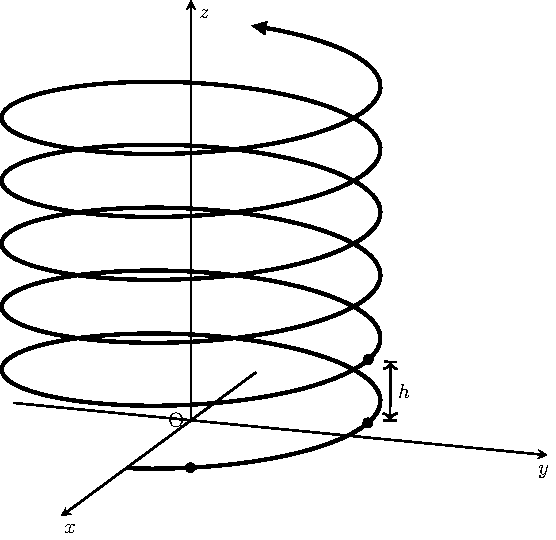
\includegraphics[width=\linewidth]{helix}
            \end{center}
        \end{minipage}
    \item Cf. ci-dessus.
    \item Soit $t_0$ un instant quelconque. Un point à ce temps-là est tel que
        \[
            \left\{
                \begin{aligned}
                    r(t_0)   & = R\\
                    \tt(t_0) & = \wt_0\\
                    z(t_0)   & = \a t_0
                \end{aligned}
            \right.
        \]
        Le premier point qui est au même angle $\tt$ mais avec $2\pi$ de plus se
        trouve donc à $t_1$ tel que
        \begin{align*}
            \tt(t_1) & = \tt(t_0) + 2\pi
            \\\Lra
            \wt_1 & = \wt_0 + 2\pi
            \\\Lra
            \Aboxed{t_1 & = t_0 + \frac{2\pi}{\w}}
        \end{align*}
        On a alors
        \vspace*{-26pt}
        \begin{gather*}
            z(t_1) - z(t_0) = h = \a t_1 - \a t_0
            \\\Lra
            \boxed{h = 2\pi \frac{\a}{\w}}
        \end{gather*}
    \item $\norm{\vf} = \sqrt{R^2\w^2+\a^2} = \cte$, donc il est uniforme. Il
        est circulaire ssi \fbox{$\a = 0$}.
    \item En regardant dans le plan polaire, on trouve $x(t)$ et $y(t)$~:
        \begin{empheq}[box=\fbox, left=\empheqlbrace]{align*}
            x(t) & = R\cos(\wt)\\
            y(t) & = R\sin(\wt)\\
            z(t) & = \a t
        \end{empheq}
\end{enumerate}

\end{document}
